\chapter{Introduction}

\section{Background}

A portable coordinate measuring arm (PCMA) is a handheld metrology instrument that captures three-dimensional (3D) coordinates directly from a physical object, as shown in ~\ref{fig:portable-coordinate-measuring-machine-arm} below, \citep{Leussink:2024}.
\begin{figure}[h!]
	\centering
	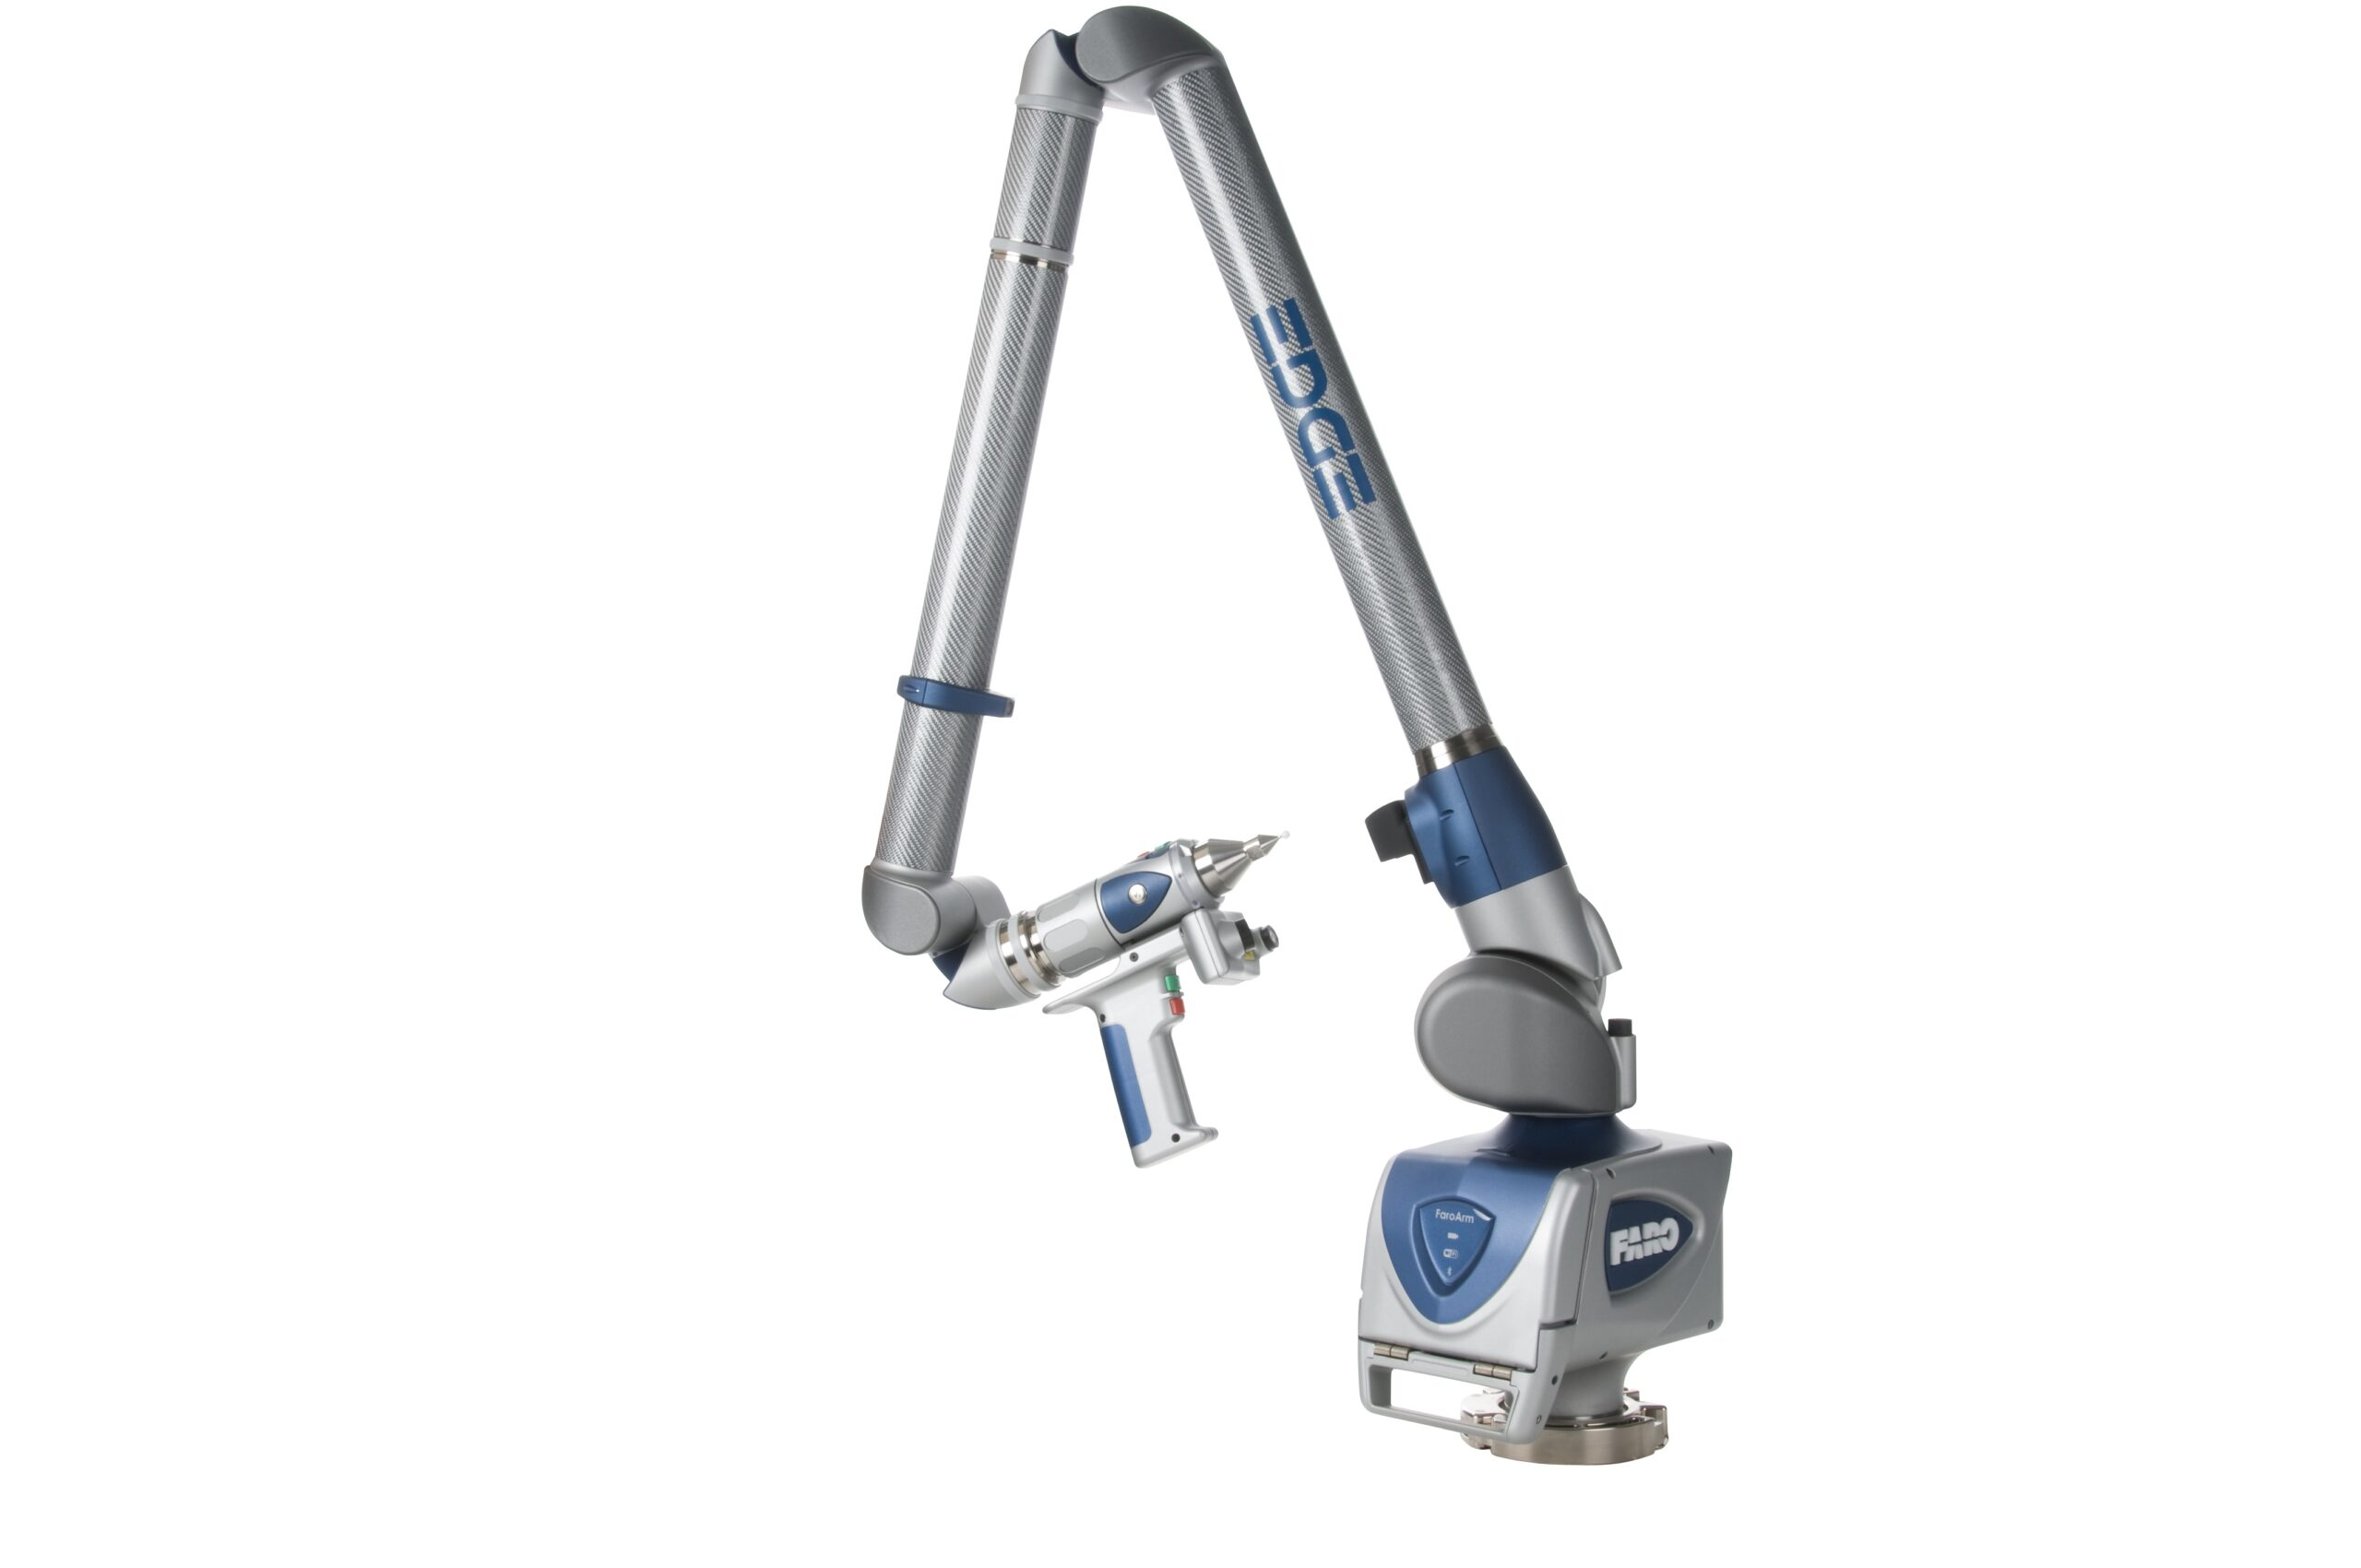
\includegraphics[width=0.6\linewidth]{../../../../../portable-coordinate-measuring-machine-arm}
	\caption[]{A portable coordinate measurement arm, \citep{Leussink:2024}}
	\label{fig:portable-coordinate-measuring-machine-arm}
\end{figure}
\\PCMAs offer adaptable measurement systems for multiple applications, such as dimensional analysis, computer-aided design (CAD) inspection, reverse engineering, etc., \citep{Ibaraki:2023}. The main limitation pf PCMAs is the effect of manual operation, which can introduce positional instability and dynamic structural deformation during measurement, \citep{Cuesta:2015}. Manual operation can also inhibit calibration procedures as it is required that the PCMA must be held still during the procedure, \citep{Rim:2019}.

\noindent As a result, designing an effective joint with a position-holding mechanism would improve the design of a PCMA and a good practice of safety. By designing the joint in this manner, error due to manual operation will be minimised, kinematic stability and accuracy will be improved.

\section{Aim and Objectives}

The aim of this project is to implement a position-holding mechanism on a PCMA without jeopardising its accuracy and ease of movement.

\noindent The objectives of the project are:
\begin{enumerate}
	\item To generalise the conventional Denavit-Hartenberg(D-H) model derived by Hall and Schreve by sampling the working volume of a PCMA determining distribution of uncertainty along its length, \citep{Hall:2010}.
	\item To design, build, and test the joint design through the single-point articulation test (SPAT), such that it maintains and/or improves the accuracy of the PCMA.
	\item To compare the results from SPAT to the D-H model and verify the joint design's effect on the PCMA's accuracy.
\end{enumerate}

\section{Scope}

In the process of determining D-H parameters, operation manual and available schematics will be used. In addition, only joint will be designed, built, and tested for data acquisition, through calibration and accuracy testing via SPAT.

\section{Motivation}

PCMAs are becoming more popular than tradition coordinate measuring machines (CMM) for in-line\footnote{In the context of PCMAs, "in-line" refers to performing quality inspections and measurements directly on the production shop floor, instead of a temperature-controlled quality laboratory, \citep{
Leussink:2024}.} and on-site industrial measurement, \citep{Leussink:2024}. They have broad applicability across multiple industries such as aerospace, automotive, heavy manufacturing, where having a portable measurement instrument decreases handling time, production delays, and revision of work.

\noindent Despite their growing popularity, the PCMA's revolute joints must satisfy competing demands, including:
\begin{itemize}
	\item Tight run-out tolerances for spatial accuracy.
	\item Sufficient holding torque to keep the arm stationary once released.
	\item Internal cable routing.
\end{itemize}
This has proved difficult since there are found commercial available joints that meet these demands.
In addition, it has been established that angular position errors at each joint propagate through the kinematic chain, which affects end-effector's accuracy, proving that joints have a measurable impact on the PCMA's accuracy, \citep{Meagher:2016}. This project addresses the gap by deriving a joint specifications from a generalised model based off of an error model that was developed by a Stellenbosch Alumnus, Leon Hall, \citep{Hall:2010}. This will produce a validated joint and testing methodology to support future PCMA development.

\section{Use of AI Tools}

Gemini is an artificial intelligence (AI) tool will be used check grammatical errors and sentence structure as well as LaTex formatting for the report.

\section{Report Overview}

This section follows the following structure:
\begin{itemize}
	\item Section 1 introduces the project background, aim and objectives, scope, and motivation for project.
	\item Section 2 presents a literature review discussing sources relevant to PCMA joint design, position-holding technology, kinematic modeling, error analysis, and PCMA testing.
	\item Section 3 details the PCMA's requirement analysis.
\end{itemize}

